

\section{Experimental Setup}

\subsection{Evaluation Platforms} We evaluate our approach on an NVIDIA RTX 2080Ti GPU, which integrates 4350 CUDA cores for floating
point computation  and 4350 CUDA cores for integer operations. The GPU has a 96KB L1 cache and shared memory. The host machine has a 2.30GHz
Intel Xeon E5-2697 CPU with 252GB memory, running Linux kernel v4.15.0. We use CUDA Toolkit version 10.2.


\subsection{Competing Methods} We compare our approach against the following state-of-the-art convolution libraries:
\begin{itemize}
  \item \textbf{cuDNN version 7.6.4}. cuDNN is a state-of-the-art convolution implementation that supports all kinds of convolutions including depthwise and pointwise convolutions on GPU. 
  Moreover, cuDNN can execute GEMM-, FFT- and Winograd-based convolutions. We take cuDNN GEMM implementation as a baseline for pointwise convolution.
  \item \textbf{Direct implementation of depthwise convolution}. We implement a direct depthwise convolution without using the proposed reuse algorithms. We take this implementation as a baseline for depthwise convolution.
\end{itemize}

\subsection{Use Cases}
We apply our approach to three depthwise convolution and pointwise convolution, described as follows.
%\mypara{2D convolution.} This applies a single-channel 2D filter to convolve the input in both horizontal and vertical
%directions in a 2D spatial domain. This is a classical and widely used 2D convolution implementation.

\mypara{Depthwise convolution.} This applies a bank of single-channel 2D filters to convolve with one multi-channel 2D input, e.g., an image of three color channels, R, G and B. We apply a 2D convolution filter to each of the input channels. 
This technique has been widely used in many CNNs, including MobileNetv2 \cite{Sandler_2018_CVPR}, EfficientNet \cite{tan2019efficientnet} and ShuffleNetv2 \cite{Ma_2018_ECCV}.

\mypara{Pointwise convolution.} This applies a bank of multi-channel 2D 1$\times$1 filters to convolve with one multi-channel 2D input. 
The 2D convolution is performed between one filter channel and the corresponding input channel, and the results are sum up across channels to generate one output channel.


\subsection{Performance Report}
We run each test case ten times under small batch sizes (1, 8, 16, 32 and 64) on an unloaded machine and report the averaged running time. 
We found little variance during execution runs, less than 2\%.  
All the convolutions used in evaluation use the standard 32-bit (single-precision) floating point numbers, and the data are organized as 4D tensors $(N,C,H,$ and $W)$, where $N$, $C$, $H$, and $W$ are the batch size, channel, height, and width, respectively. 
In this work, we first test depthwise convolution with two filter sizes, $3 \times 3$ and $5 \times 5$, because these are commonly used filter sizes. 
Then we report the performance of pointwise convolution. 
Lastly, we apply our optimized depthwise and pointwise convolutions on MobileNetv2 and report the performance of inference.
%
%\subsection{Notations}
%Throughout the evaluation, we use $I$, $F$, and $O$ to represent the input, the filter, and the output respectively, $N$, $C$, $H$, and $W$
%to denote the batch size, the channel, the height, and the width, respectively.

\section{Experimental Results}
\label{exp} In this section, we report our results for depth-wise convolution (Section \ref{sec:depconvexp}), pointwise convolution (Section \ref {multicconvexp}) and inference of MobileNetv2 showing that our approach consistently outperforms alternative methods by delivering the overall best performance.


%\subsection{2D Convolution\label{sec:ex2dc}}
%\begin{figure*}
%\centering
%\subfloat[][$3 \times 3$ filter]{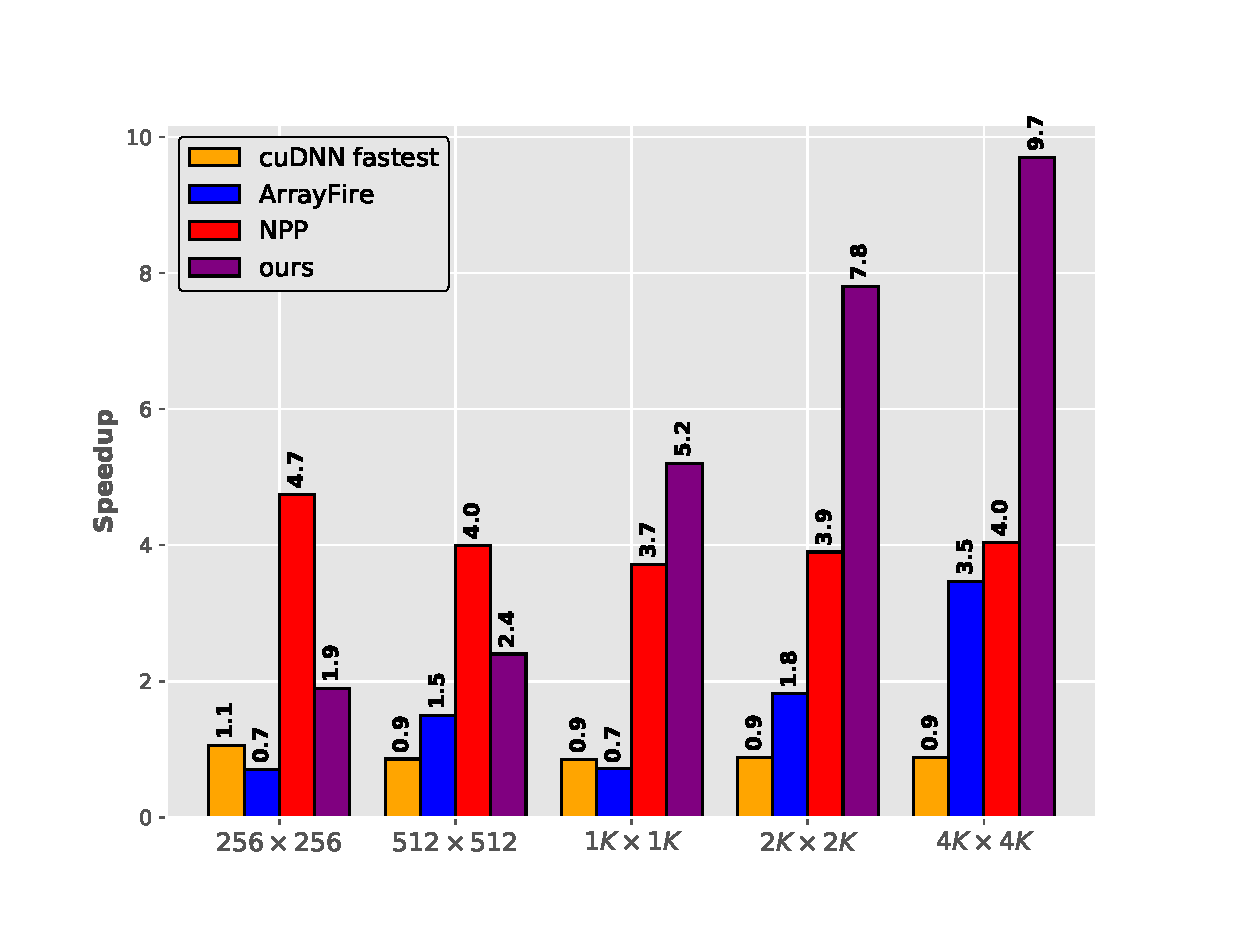
\includegraphics[width=0.85\columnwidth]{./figure/2d_conv_f3.eps}
%	\label{fig:2druntimef3c12080}}
%\hspace{0em}
%\subfloat[][$5 \times 5$ filter]{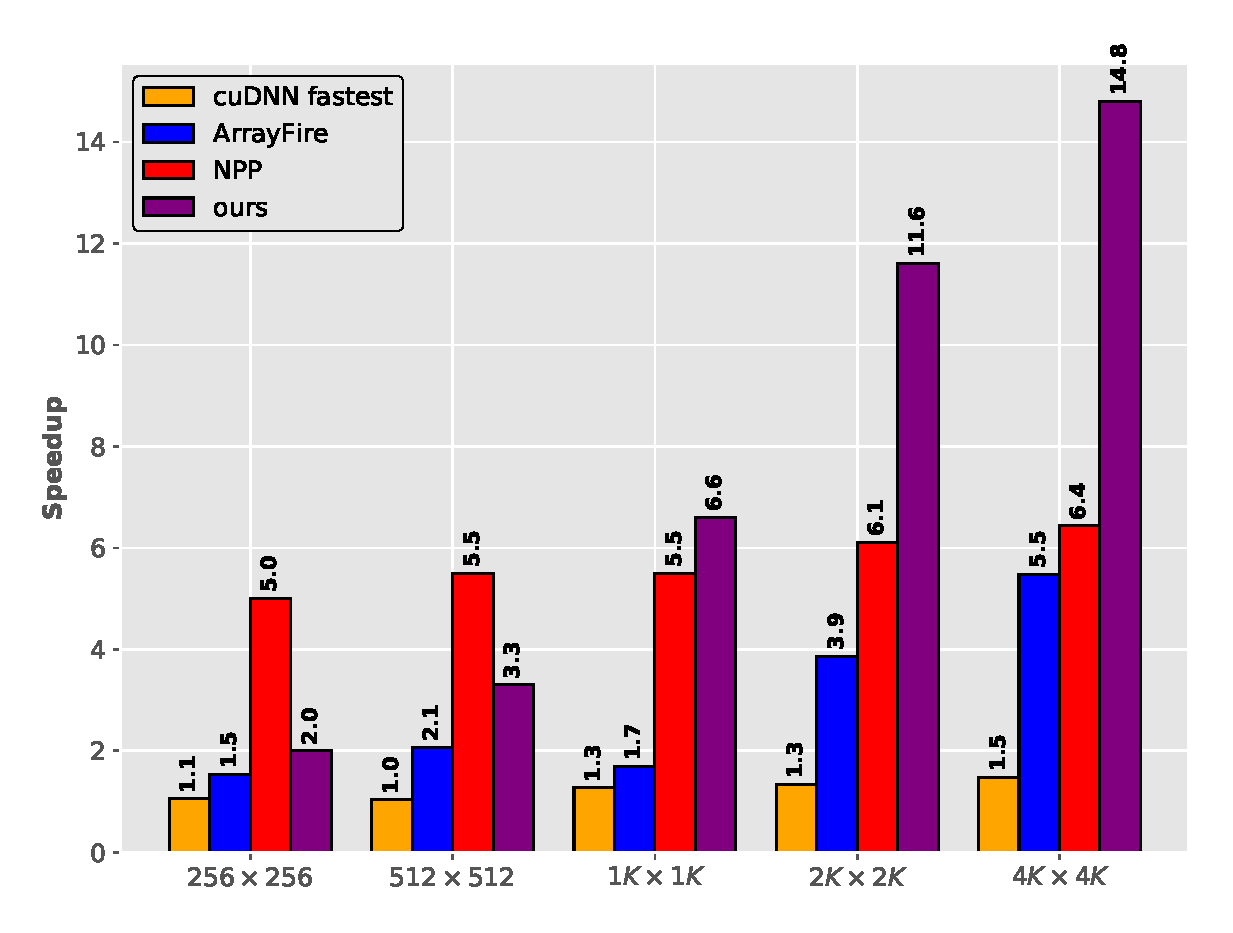
\includegraphics[width=0.85\columnwidth]{./figure/2d_conv_f5.eps}
%	\label{fig:2druntimef5c12080}}
%
%\vspace{-1mm}	\caption{Speedups of 2D convolutions of four implementations over GEMM-im2col when using a $3 \times 3$ (a) and a $5 \times
%5$ filter (b).} \label{fig:2druntime} \vspace{-3mm}
%\end{figure*}
%
%
%\subsubsection{Setup}
%In this experiment, we compare our approach against the 2D convolution implementations from cuDNN, GEMM-im2col, ArrayFire, and
%NPP. As cuDNN provides multiple implementations, we empirically choose the fastest version, denoted as cuDNN-fastest, for evaluation. We
%apply each method to images with sizes ranging from $256 \times 256$ to $4K \times 4K$. We set the batch size, channel, height, and width
%of the input to be 1.
%
%
%\subsubsection{Overall results}
% Figure
%\ref{fig:2druntime} reports the speedups of cuDNN, ArrayFire, NPP and our approach over GEMM-im2col. While cuDNN has been heavily optimized
%for NVIDIA GPUs, it does not show a notable performance advantage. When using a $3 \times 3$ filter, our approach gives the best overall
%speedup of 5.4$\times$ (up to 9.7$\times$ for the largest input), which translates to an improvement of  more than 30\% over the second-best method, NPP.
%We note that our approach is based on the standard 2D direct convolution by applying the column and row reuse algorithms. Therefore, the
%performance gain is mainly attributed to the reduction of the number of memory transactions. When using a $5 \times 5$ filter, our approach
%achieves a better overall speedup of $7.7\times$. A $5 \times 5$ filter has four overlapped columns and rows (instead of just one
%overlapped column and row on width and height dimensions when using a $3 \times 3$ filter). The larger number of overlapped data thus gives
%more room for performance optimization when using our column and row reuse algorithms. Our approach achieves the best overall performance
%and demonstrates significant performance advantages when processing large input.
%
%\subsubsection{Further analysis}
%\begin{figure}[t!]
%\centering
%
%\subfloat[][Memory throughput]{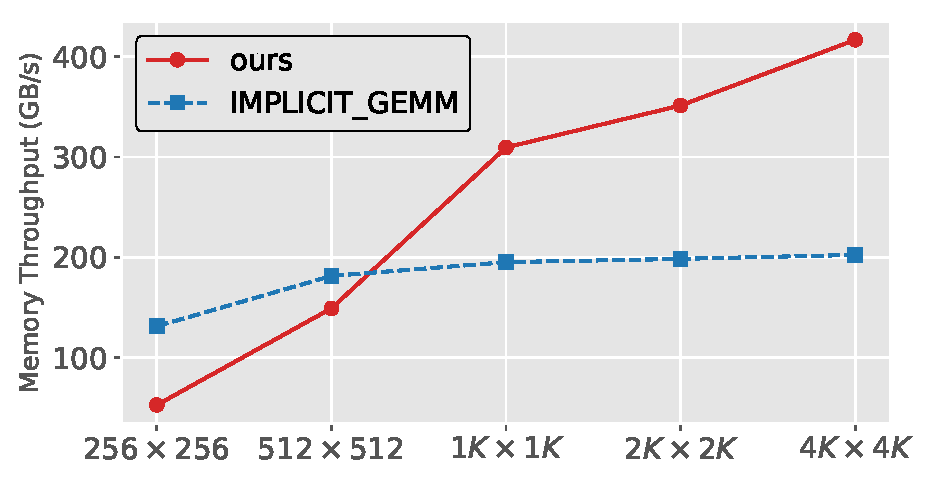
\includegraphics[width=0.85\columnwidth]{./figure/2dmemthroughput.eps}
%	\label{fig:2dmemthr}}
%
%\subfloat[][Maximum bandwidth]{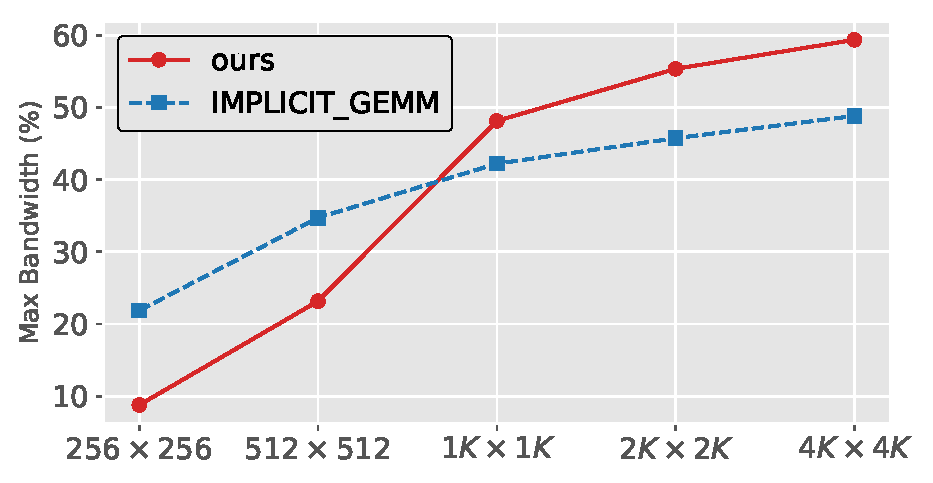
\includegraphics[width=0.85\columnwidth]{./figure/2dmembandwidth.eps}
%	\label{fig:2dmaxband}}
%	
%\caption{Memory throughput (a) and maximum bandwidth (b) of NPP and our implementation for the filter of size $3 \times 3$.}
%\label{fig:2dmemanaly}
%\vspace{-5mm}
%\end{figure}
%
%On the test cases of small input sizes (i.e., $256 \times 256$ and $512 \times 512$), NPP gives the best performance. To understand the
%performance gap on small input sizes, we use \emph{nvidia compute} to collect memory profiles, including memory throughput and max
%bandwidth, of our implementation and NPP when using a $3 \times 3$ filter to perform convolution. The profiling results are shown in Figure
%\ref{fig:2dmemanaly}.  We see that as the input size increases, the memory throughput and the maximum bandwidth also grow. This is expected
%as the larger the input image, the larger number the memory transactions is likely to be when performing convolution.  We also observe that
%our approach leads to higher memory throughput and the maximum bandwidth used when the input image size is greater or equal than $1K \times
%1K$. This finding matches the results presented in Figure \ref{fig:2druntime}, where our approach gives the best performance when
%processing an image whose size is $1K \times 1K$ or larger. This result also suggests that memory performance has a strong correlation with
%the performance of 2D convolutions.
%
%
%The reason why our approach gives lower memory throughput and achieves lower maximum bandwidth on small input sizes over NPP is explained
%as follows. For 2D convolution, only one filter is used to convolve with one single-channel input feature map, which
%requires much less computation compared to, e.g., the depth-wise or multi-channel 2D convolutions. Therefore, memory performance has a huge
%impact on the performance of 2D convolutions. Our row reuse algorithm performs better when a thread operates on more rows of output.
%However, the more rows a thread compute on, the fewer warps and thread blocks we can generate. Without enough warps issuing memory
%requests, the memory throughput and maximum bandwidth will reduce significantly, which leads to slower performance over NPP. As the input
%size increases, we can allocate more thread blocks and more warps per thread block. With enough memory requests and a reduction in redundant
%memory transactions, we can increase the memory throughput and max bandwidth to improve the performance of 2D convolutions.
%
%\subsubsection{Summary} Overall, our optimization algorithms can greatly reduce the number of memory transactions and improve the performance of 2D
%convolutions. Compared with state-of-the-art image processing libraries, NPP, our approach achieves average speedups of 1.4$\times$ and
%1.3$\times$ when using a $3 \times 3$ and $5 \times 5$ filters, respectively.

\subsection{Depthwise Convolution}
\label{sec:depconvexp}

\begin{table}[]
\caption{Layer configurations of depthwise  convolutions$^{\dag}$.}
\label{tab:depconvconfigs}
\centering
\rowcolors{2}{}{Gray}
\begin{threeparttable}
\begin{tabular}{lrrrrr}
\toprule
& \textbf{$I_N$} & \textbf{$I_C$} & \textbf{$I_H \times I_W$ }&  \textbf{$F_H \times F_W$} &\textbf{$S$}\\
\midrule
\textbf{CONV1} & 1,8,16,32,64,128  & 16    & 112$\times$112 & $3 \times 3$, $5 \times 5$&2  \\
\textbf{CONV2} & 1,8,16,32,64,128  & 72    & 56$\times$56  &$3 \times 3$, $5 \times 5$  &2 \\
\textbf{CONV3} & 1,8,16,32,64,128  & 88   & 28$\times$28  &$3 \times 3$, $5 \times 5$   &1 \\
\textbf{CONV4} & 1,8,16,32,64,128  & 96    & 28$\times$28  &$3 \times 3$, $5 \times 5$  &2  \\
\textbf{CONV5} & 1,8,16,32,64,128  & 96   & 14$\times$14  &$3 \times 3$, $5 \times 5$   &1 \\
\textbf{CONV6} & 1,8,16,32,64,128  & 120   & 14$\times$14  &$3 \times 3$, $5 \times 5$  &1  \\
\textbf{CONV7} & 1,8,16,32,64,128  & 192   & 14$\times$14  &$3 \times 3$, $5 \times 5$  &1  \\
\textbf{CONV8} & 1,8,16,32,64,128  & 240   & 14$\times$14  &$3 \times 3$, $5 \times 5$  &2  \\
\textbf{CONV9} & 1,8,16,32,64,128  & 432   & 7$\times$7  &$3 \times 3$, $5 \times 5$    &1\\

\bottomrule
\end{tabular}
\footnotesize
\begin{tablenotes}
\item[\dag] We use $I$, $F$, $O$ and $S$ to represent the input, the filter, the output and the stride respectively, $N$, $C$, $H$, and $W$
to denote the batch size, the channel, the height, and the width, respectively.
\end{tablenotes}
\end{threeparttable}
\vspace{-5mm}
\end{table}

\begin{figure*}
\centering
	
\subfloat[][$3\times 3$ filter]{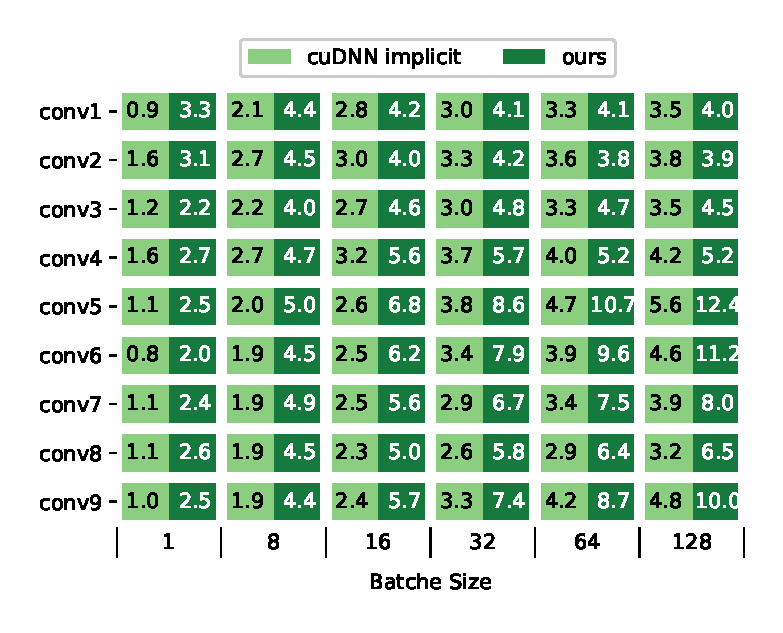
\includegraphics[width=\columnwidth]{./figure/depthwise_speedup_3f.eps}
	\label{fig:f3dwruntime2080}}
\subfloat[][$5\times 5$ filter]{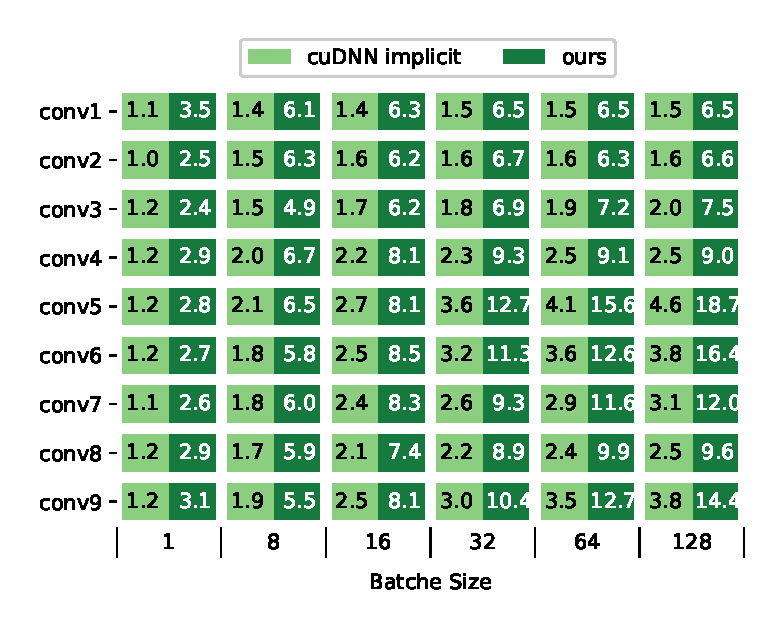
\includegraphics[width=\columnwidth]{./figure/depthwise_speedup_5f.eps}
	\label{fig:f5dwruntime2080}}

\vspace{-2mm} \caption{Speedups of our approach and cuDNN over the baseline implementation of the depthwise convolution when using a
$3\times 3$ (a) and a $5\times 5$ filter (b).} \label{fig:dwruntime}
\vspace{-2mm}
\end{figure*}


\subsubsection{Setup} In this experiment, we compare our approach against the depthwise convolution implementations of cuDNN. Specifically, we compare to seven algorithms in cuDNN, including IMPLICIT\_GEMM (implicit), IMPLICIT\_PRECOMP\_GEMM (precomp), GEMM (gemm), FFT (fft), FFT\_TILING (tiling), WINOGRAD (winograd) and WINOGRAD\_NONFUSED (nonfused). 
As the fastest algorithm of cuDNN is always implicit, we only report the performance of implicit algorithm. 
As a baseline, we implement a simple depthwise convolution. 
We use the convolutional layer configurations that apply depthwise convolution from the popular CNN model, MobileNetv2. 
We report the performance when the input and output batch
sizes are set to 1, 8, 16, 32, 64 and 128. 
Table \ref{tab:depconvconfigs} gives the layer configurations used in this experiment.

%In the depth-wise convolution, one input element only needs to be convolved with one filter, while in the multi-channel 2D convolution, one input element needs to be convolved with all filters. 
%Therefore, depth-wise convolutions require much less computation than multi-channel 2D convolutions, which makes depth-wise convolutions more sensitive to memory performance.
%Nowadays, depth-wise convolutions have been widely used in embedded CNNs, including MobileNetv2 \cite{Sandler_2018_CVPR}, EfficientNet \cite{tan2019efficientnet} and ShuffleNetv2 \cite{Ma_2018_ECCV}. 
%In this section, we present the performance comparison of the depth-wise convolution between cuDNN and our implementation. 
%We implement a simple depth-wise convolution and report speedups of cuDNN and our implementation over the simple depth-wise convolution. 
%We evaluate 7 algorithms in cuDNN, including IMPLICIT\_GEMM (implicit), IMPLICIT\_PRECOMP\_GEMM (precomp), GEMM (gemm), FFT (fft), FFT\_TILING (tiling), WINOGRAD (winograd) and WINOGRAD\_NONFUSED (nonfused).
%Winograd can not be applied on a $5 \times 5$ filter, thus we set speedups for this algorithm to 0.
%We collect configurations of the convolutional layers using depth-wise convolution from three popular mobile embedded models,
%namely, MobileNetv2, ShuffleNetv2 and EfficientNet.
%Then, we set the number of the batch size to 512 ($I_N=O_N=512$). Other batch sizes demonstrate a similar performance because all tested implementations have a linear scale as the batch size. The exact configuration is presented in Table \ref{tab:3dconvconfigs}.

\subsubsection{Overall results}
Figure \ref{fig:dwruntime} shows that our approach gives the best speedups. 
Our approach delivers an average speedup of $5.4\times$ and $7.8\times$ for the $3 \times 3$ and $5 \times 5$ filters, respectively. 
The implicit algorithm achieves an average speedup of $2.8\times$ and $2.1\times$ for the $3 \times 3$ and $5 \times 5$ filters, respectively.
Other algorithms of cuDNN except implicit algorithm perform poorly in all test cases. 
Since that cuDNN is a closed source, we cannot investigate the source code for further analysis. 
We hypothesize that FFT- and Winograd- based algorithms focus on the reduction of computation and trades memory performance for speed. 
Precomp and gemm algorithms need extra memory operations to compute output elements. 
Moreover, depthwise convolution is more sensitive to memory performance than pointwise and multi-channel 2D convolutions. 
Consequently, these algorithms are not suitable for depthwise convolutions. 
Overall, our approach improves implicit by $1.9\times$ (up o $3.5\times$) and $3.5\times$ (up to $4.4\times$) when using a $3 \times 3$ and $5 \times 5$ filter respectively.
%When using a $5 \times 5$ filter, our approach achieves a better overall speedup of $7.7\times$. A $5 \times 5$ filter has four overlapped columns and rows (instead of just one
%overlapped column and row on width and height dimensions when using a $3 \times 3$ filter). The larger number of overlapped data thus gives
%more room for performance optimization when using our column and row reuse algorithms. 
%The algorithms of cuDNN except implicit algorithm perform poorly in all test cases and the speedups of these algorithms all below 1.
%Considering that cuDNN is a closed source, we can only guess that FFT- and Winograd- based algorithms focus on reduction of computation and
%trades memory performance for speed. Precomp and gemm algorithms need extra memory operations to compute output elements. Moreover,
%depth-wise convolution is more sensitive to memory performance than multi-channel 2D convolution. Consequently, these algorithms perform
%poorly on depth-wise convolutions.
\begin{figure}
    \centering
    \subfloat[][Ratios of SM utilization of implicit and ours to the sum of both utilizations.]{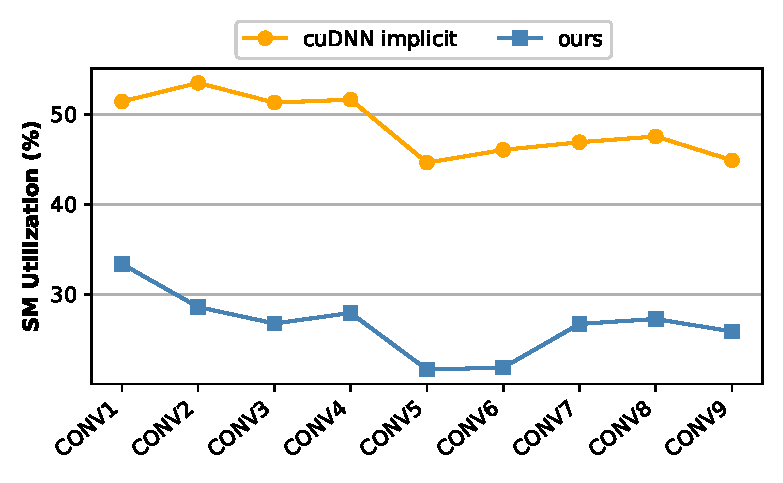
\includegraphics[width=0.9\columnwidth]{./figure/smutil.eps}\label{fig:dwsmutil}}
    \qquad
    \vspace{5mm}
    \subfloat[][Ratios of executed LDG (load from global memory) instruction counts of implicit and ours to the sum of both counts.]{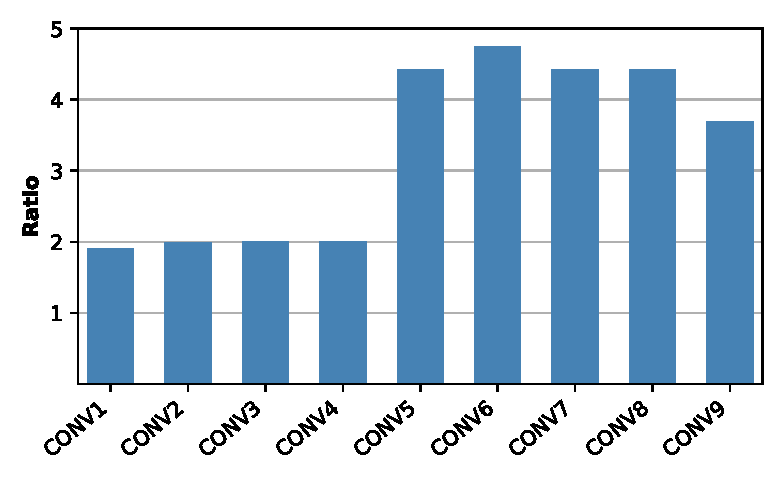
\includegraphics[width=0.9\columnwidth]{./figure/ldginst.eps}\label{fig:dwldginst}}
    \vspace{-4mm}
    \caption{LDG instruction counts and SM utilization of depthwise convolutions with a batch size of 32 and a filter size of $3\times3$. 
    Other configurations have the similar ratios.}
    \label{fig:dwratio}
\end{figure}

\subsubsection{Further analysis}
We note that our approach is based on the standard 2D direct convolution by applying the column and row reuse algorithms. 
Therefore, the performance gain is mainly attributed to the reduction of the number of memory operations. 

Figure \ref{fig:dwratio} reports the measured LDG (load from global memory) instruction counts and SM utilization for the fast cuDNN implicit algorithm and our approach when using a $3 \times 3$ filter and a batch size of 32. Other configurations have the similar performance. 
We can see in Figure \ref{fig:dwsmutil} that cuDNN implicit algorithm has an average of $2\times$ higher SM utilization compared our approach.
The reason why our approach gives lower SM utilization as follows. 
Our row reuse algorithm performs better when a thread operates on more rows of output.
However, the more rows a thread compute on, the fewer warps and thread blocks we can generate. Without enough warps running on SMs, the SM utilization will reduce significantly.
Though cuDNN implicit has high SM utilization, it does not achieve a good performance for depthwise convolution. 
The reason is that depthwise convolution possesses a very low arithmetic intensity (as described in Section) and is more sensitive to memory performance.
In contrary to cuDNN implicit, we focus on optimizing memory performance and uses row and column reuse techniques to reduce memory operations by a maximum of $9\times$ lower executed LDG instructions, as shown in Figure \ref{fig:dwldginst}.
This suggests that our reuse algorithms can improve memory performance significantly, which thus leads to better computational performance.

\subsubsection{Summary}
Our approach can significantly reduce the number of memory operations and improve the memory performance, which leads to faster computation time when performing
depth-wise convolutions.  Compared to the fastest available algorithms in cuDNN, which is the state-of-the-art convolution library, our
approach achieves an average speedup of $1.9\times$ and $3.5\times$ when using a $3 \times 3$ and $5 \times 5$ filter, respectively.


\subsection{Pointwise Convolution}
\label{sec:pwconvexp}

\begin{table}[]
\caption{Layer configurations used for pointwise 2D convolutions$^{\dag}$.}
\label{tab:pwconv}
\rowcolors{2}{}{Gray}
\begin{threeparttable}
\begin{tabular}{lrrrrr}
\toprule
& \textbf{$I_N$} & \textbf{$I_C=F_C$} & \textbf{$I_H \times I_W$} & \textbf{$F_N$} & \textbf{$F_H \times F_W$} \\
\midrule
\textbf{CONV1}  & 1,8,16,32,64,128  & 16    & $56\times 56$   & 8   & $1\times 1$\\
\textbf{CONV2}  & 1,8,16,32,64,128  & 8     & $56\times 56$   & 16  & $1\times 1$\\
%\textbf{CONV3}  & 1,8,16,32,64,128  & 16    & $56\times 56$   & 16  & $1\times 1$\\
\textbf{CONV4}  & 1,8,16,32,64,128  & 16    & $56\times 56$   & 72  & $1\times 1$\\
\textbf{CONV5}  & 1,8,16,32,64,128  & 72    & $28\times 28$   & 24  & $1\times 1$\\
%\textbf{CONV6}  & 1,8,16,32,64,128  & 24    & $28\times 28$   & 88  & $1\times 1$\\
%\textbf{CONV7}  & 1,8,16,32,64,128  & 88    & $28\times 28$   & 24  & $1\times 1$\\
\textbf{CONV8}  & 1,8,16,32,64,128  & 24    & $28\times 28$   & 96  & $1\times 1$\\
\textbf{CONV9}  & 1,8,16,32,64,128  & 96    & $14\times 14$   & 24  & $1\times 1$\\
\textbf{CONV10} & 1,8,16,32,64,128  & 24    & $14\times 14$   & 96  & $1\times 1$\\
%\textbf{CONV11} & 1,8,16,32,64,128  & 96    & $14\times 14$   & 32  & $1\times 1$\\
\textbf{CONV12} & 1,8,16,32,64,128  & 32    & $14\times 14$   & 192 & $1\times 1$\\
\textbf{CONV13} & 1,8,16,32,64,128  & 192   & $14\times 14$   & 48  & $1\times 1$\\
%\textbf{CONV14} & 1,8,16,32,64,128  & 48    & $14\times 14$   & 192 & $1\times 1$\\
%\textbf{CONV15} & 1,8,16,32,64,128  & 192   & $14\times 14$   & 32  & $1\times 1$\\
%\textbf{CONV16} & 1,8,16,32,64,128  & 32    & $14\times 14$   & 96  & $1\times 1$\\
\textbf{CONV17} & 1,8,16,32,64,128  & 96    & $14\times 14$   & 40  & $1\times 1$\\
\textbf{CONV18} & 1,8,16,32,64,128  & 40    & $14\times 14$   & 120 & $1\times 1$\\
\textbf{CONV19} & 1,8,16,32,64,128  & 120   & $14\times 14$   & 32  & $1\times 1$\\
%\textbf{CONV20} & 1,8,16,32,64,128  & 32    & $14\times 14$   & 120 & $1\times 1$\\
%\textbf{CONV21} & 1,8,16,32,64,128  & 120   & $14\times 14$   & 40  & $1\times 1$\\
\textbf{CONV22} & 1,8,16,32,64,128  & 40    & $14\times 14$   & 240 & $1\times 1$\\
\textbf{CONV23} & 1,8,16,32,64,128  & 240   & $7\times 7$     & 64  & $1\times 1$\\
\textbf{CONV24} & 1,8,16,32,64,128  & 64    & $7\times 7$     & 240 & $1\times 1$\\
%\textbf{CONV25} & 1,8,16,32,64,128  & 240   & $7\times 7$     & 72  & $1\times 1$\\
\textbf{CONV26} & 1,8,16,32,64,128  & 72    & $7\times 7$     & 432 & $1\times 1$\\
\textbf{CONV27} & 1,8,16,32,64,128  & 432   & $7\times 7$     & 112 & $1\times 1$\\
\textbf{CONV28} & 1,8,16,32,64,128  & 112   & $7\times 7$     & 432 & $1\times 1$\\
\textbf{CONV29} & 1,8,16,32,64,128  & 432   & $7\times 7$     & 72  & $1\times 1$\\
\textbf{CONV30} & 1,8,16,32,64,128  & 432   & $7\times 7$     & 1024& $1\times 1$\\

\bottomrule
\end{tabular}
\begin{tablenotes}
\item[\dag] We use $I$, $F$, and $O$ to represent the input, the filter, and the output respectively, $N$, $C$, $H$, and $W$
to denote the batch size, the channel, the height, and the width, respectively.
\end{tablenotes}
\end{threeparttable}
\end{table}

\begin{figure}
\centering
	
\subfloat{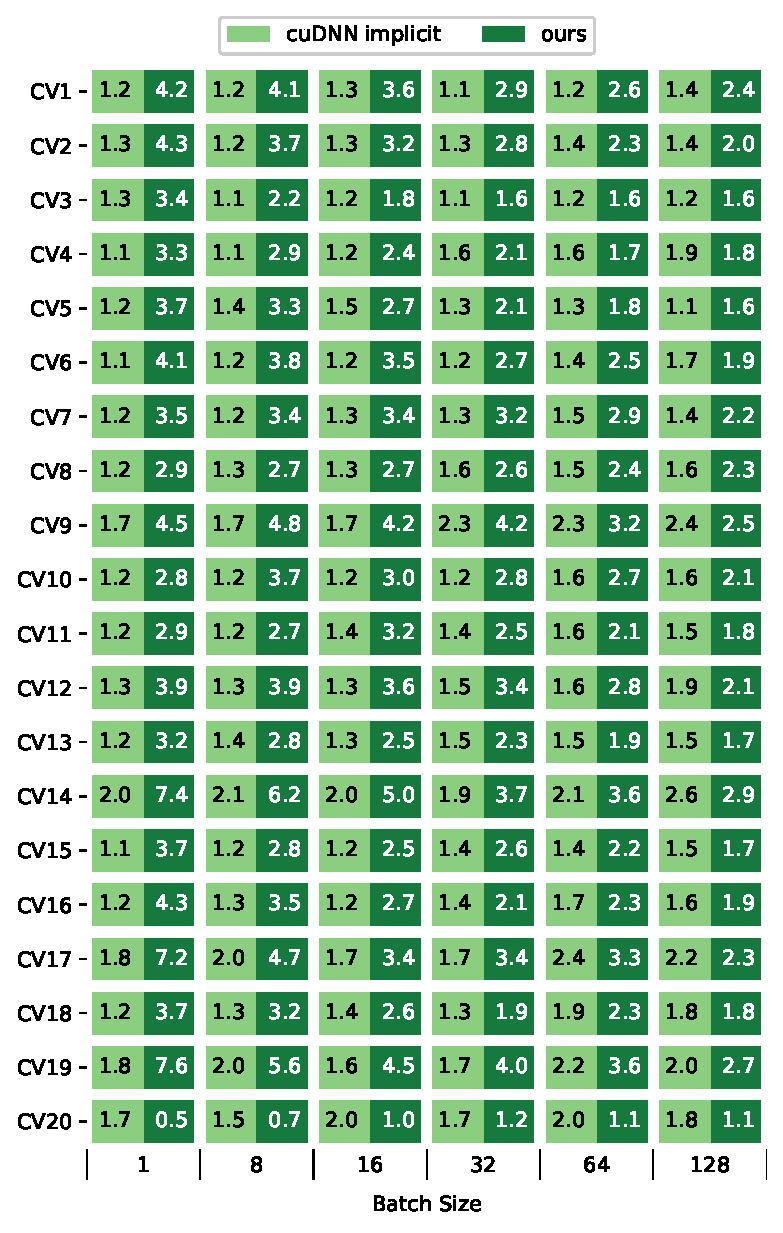
\includegraphics[width=0.9\columnwidth,height=13cm]{./figure/pwexectime.eps}}
\vspace{-2mm}
\caption{Speedups of our approach and cuDNN over cuDNN gemm} \label{fig:pwexectime}
\vspace{-5mm}
\end{figure}


\subsubsection{Setup} In this experiment, we compare our approach against the pointwise convolution implementations in cuDNN and use cuDNN gemm as the baseline. 
We use the layer configurations from the popular CNN model MobileNetv2.
There are 30 different configurations for pointwise convolfution, we test all configurations and report the performance of 20 layers to reduce the space. Unchoosen layers have the similar performance as choosen ones.  
We report the performance when the input and output batch sizes are set to 1, 8, 16, 32, 64 and 128.
In all configurations of pointwise convolution, cuDNN implicit performs best among all algorithms in cuDNN, therefore we only show the results of cuDNN implicit.
Table \ref{tab:pwconv} lists the layer configurations used in this experiment.

\subsubsection{Overall results} Figure \ref{fig:pwexectime} shows the speedups of cuDNN implicit and our approach over cuDNN gemm.
Our approach achieves the best performance for CONV1-CONV? convolutions.
For CONV?, which uses 1024 filters to convolve with the input, our approach performs poorly compared to cuDNN gemm and cuDNN implicit.
Overall, our implementation achieves an average speedup of ?$\times$ and ?$\times$ over cuDNN gemm. 
This translates to an improvement of ?$\times$ over the fastest algorithm in cuDNN.

\subsubsection{Further analysis}
\begin{figure}
    \centering
    \subfloat[][Ratios of SM utilization of implicit and ours to the sum of both utilizations.]{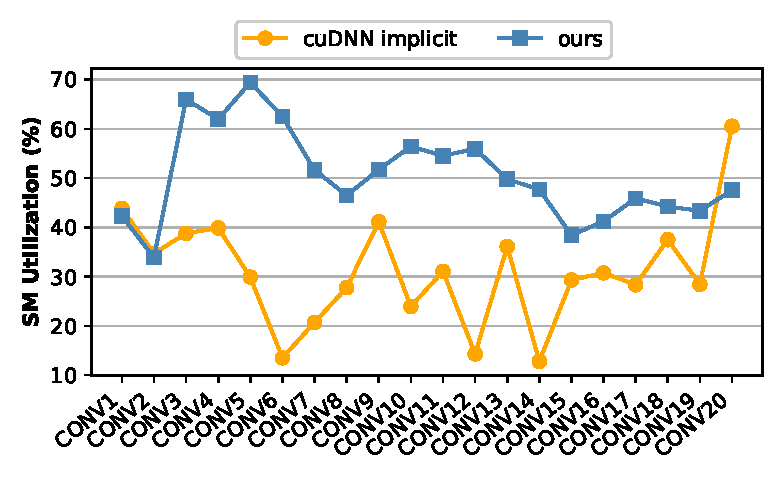
\includegraphics[width=0.9\columnwidth]{./figure/pwsmutil.eps}\label{fig:pwsmutil}}
    \qquad
    \vspace{5mm}
    \subfloat[][Ratios of executed LDG (load from global memory) instruction counts of implicit and ours to the sum of both counts.]{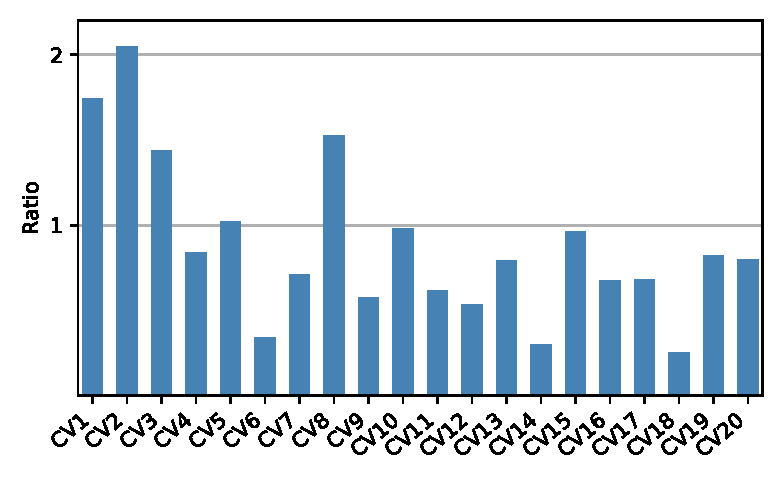
\includegraphics[width=0.9\columnwidth]{./figure/pwldginst.eps}\label{fig:pwldginst}}
    \vspace{-4mm}
    \caption{LDG instruction counts and SM utilization of pointwise convolutions with a batch size of 32. 
    Other configurations have the similar ratios.}
    \label{fig:pwratio}
\end{figure}
Figure \ref{fig:pwratio} reports the measured LDG (load from global memory) instruction counts and SM utilization for the cuDNN implicit algorithm and our approach when using a batch size of 32. Other configurations have the similar performance. 

Given a specific layer configuration of pointwise convolution, our approach will create more thread blocks, which leads to a higher SM utilization, and also keeps a certain amount of computation for each thread to hide global memory access laytency.
We can see in Figure \ref{fig:pwsmutil} that out approach has an average of $1.9\times$ higher SM utilization compared to cuDNN implicit. 
The performance gain of our approach is mainly attributed to the hgiger SM utilization.
As can be seen in Figure \ref{fig:pwldginst}, the number of executed LDG instructions of our approach is ?$\times$ higher than cuDNN implicit. 
The reason is that we create more thread blocks and the input or the filter which is shared by multiple thread blocks will be loaded multiple times, therefore our approach will have a higher LDG instruction count than cuDNN implicit.
But this sideeffect will be eleminated by the increased SM utilization.


\begin{figure*}
    \centering
    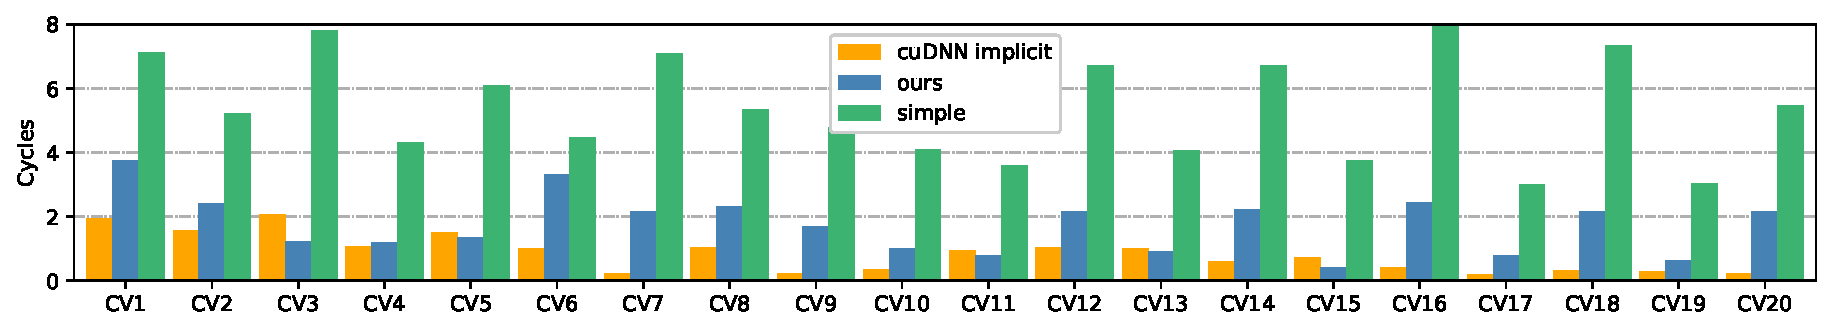
\includegraphics[width=0.97\textwidth,height=4.5cm]{./figure/longscore.eps}
    \caption{The average number of cycles each warp spends on waiting for the global operation to complete.}
    \label{fig:stalllongscore}
\end{figure*}


\subsection{Inference Performance}
\subsubsection{Setup} In this experiment, we apply our depthwise and pointwise convolutions on the inference of MobileNetv2 for batch sizes of 1, 8, 16, 32, 64 and 128.
We use caffe framework to implement MobileNetv2 and made some modifications to the source code of caffe before performing experiments. 
First, we replace the implementation of batchnormalization and depthwise convolffution layers with cuDNN implementations. 
To perform the experiment, we first run the inference with cuDNN implementation and then replace the cuDNN with our implemnetation.
We test using batch sizes of 1, 8 16, 32, 64 and 128 and record the end-to-end runtime.
\subsubsection{Overall result}
\begin{table}[]
    \caption{Experiments for inference using MobileNetv2}
    \label{tab:infertime}
    \centering
    \rowcolors{2}{}{Gray}
    \begin{threeparttable}
    \begin{tabular}{l|rrrrrr}
    \toprule
    \textbf{batch} size& 1 & 8 & 16& 32 &64 & 128\\
    \midrule
    \textbf{implicit} & 10.50  & 11.57 & 16.68 & 25.81 &46.23 &69.67  \\
    \textbf{ours} &8.89   &9.81    & 14.68  & 23.3 &40.12 &64.33 \\
    \textbf{improvement(\%)} &15.33   &15.21    & 11.99  & 9.72 &13.22 &7.66 \\
    
    \bottomrule
    \end{tabular}
    \footnotesize
    \end{threeparttable}
    \vspace{-5mm}
\end{table}
Table \ref{tab:infertime} demonstrates that our approach improves the performance of inference by 12.19\% on average compared to the implementation of cuDNN implicit.